\chapter{神经系统疾病}

\chapterabstract{本章主要介绍中枢神系统几种常见的感染性疾病和变性疾病。要求掌握流行性脑脊髓膜炎和流行性乙型脑炎的形态学特征及其鉴别要点;熟悉流行性脑脊髓膜炎和流行性乙型脑炎的临床病理联系、结局及并发症,阿尔茨海默病和帕金森病的病理变化及临床病理联系;了解各神经系统疾病的病因与发病机制。}

\section{流行性脑脊髓膜炎}

流行性脑脊髓膜炎(epidemic cerebrospinal
meningitis)是由脑膜炎双球菌引起的急性传染病,简称流脑。病变主要在大脑软脑膜,脊髓膜也可受累,病理特征是脑、脊髓膜的急性化脓性炎症。临床表现为发热、头痛、呕吐、皮肤及黏膜淤点淤斑,颅内压增高和脑膜刺激症状。好发于儿童和青少年,多为散发性,冬春季节可以发生流行。

\subsection{病因及发病机制}

脑膜炎双球菌为革兰阴性菌,其荚膜能抵抗白细胞的吞噬作用,菌体裂解后释放出的内毒素能造成小血管或毛细血管出血和坏死,为其主要的致病因素。该菌存在于病人或带菌者的鼻咽部,由飞沫经呼吸道传染。细菌侵入上呼吸道后,大多数人不发病或仅有轻度局部卡他性炎,成为健康带菌者。若机体抵抗力低下或细菌数量多、毒力强,细菌在局部大量繁殖并侵入血液,可引起短期菌血症或败血症,仅少数人(2%~3%)因内毒素作用,细菌可突破血脑屏障,到达脑脊髓膜,引起急性化脓性脑脊髓膜炎。

\subsection{病理变化}

根据病变发展过程,典型的可分为四期,病变特点如下:

\subsubsection{上呼吸道感染期}

细菌在鼻咽部黏膜繁殖,引起鼻咽部轻度卡他性炎,黏膜充血、水肿,少量中性粒细胞浸润,分泌物增多。此期持续1~2天。

\subsubsection{败血症期}

机体抵抗力低下时,细菌进入血液,繁殖并产生内毒素引起败血症。约有70%病人皮肤和黏膜出现淤点或淤斑,严重者淤斑迅速扩大中央可发生坏死,之后形成溃疡,这是由于小血管被细菌栓塞以及毒素对血管壁的损伤所致,是本期的特征性表现。此期血培养阳性,出血处刮片80%病例可找到细菌。此期持续1~2天。

\subsubsection{脑脊髓膜炎症期}

主要病变是脑脊髓膜的化脓性炎症。此期一般持续2~5天。

\paragraph{肉眼观}
脑脊髓膜血管高度扩张充血,蛛网膜下隙特别是脑沟血管周围充满黄色脓性渗出物,严重时覆盖脑沟脑回使其结构不易辨认(图\ref{fig13-1}a)。病变一般以大脑额叶和顶叶的表面、脑底部最明显,其他部位如小脑的脑膜、脊髓膜、颅神经和脊神经均可累及。脑室内常含有混浊的液体或脓液。

\paragraph{镜下观}
蛛网膜下隙充满大量中性粒细胞、少量淋巴细胞、巨噬细胞和纤维素,血管高度扩张、充血(图\ref{fig13-1}b)。脑实质一般无明显改变,严重病例邻近脑膜的脑实质也可出现明显炎症(脑膜脑炎)。

\begin{figure}[!htbp]
 \centering
 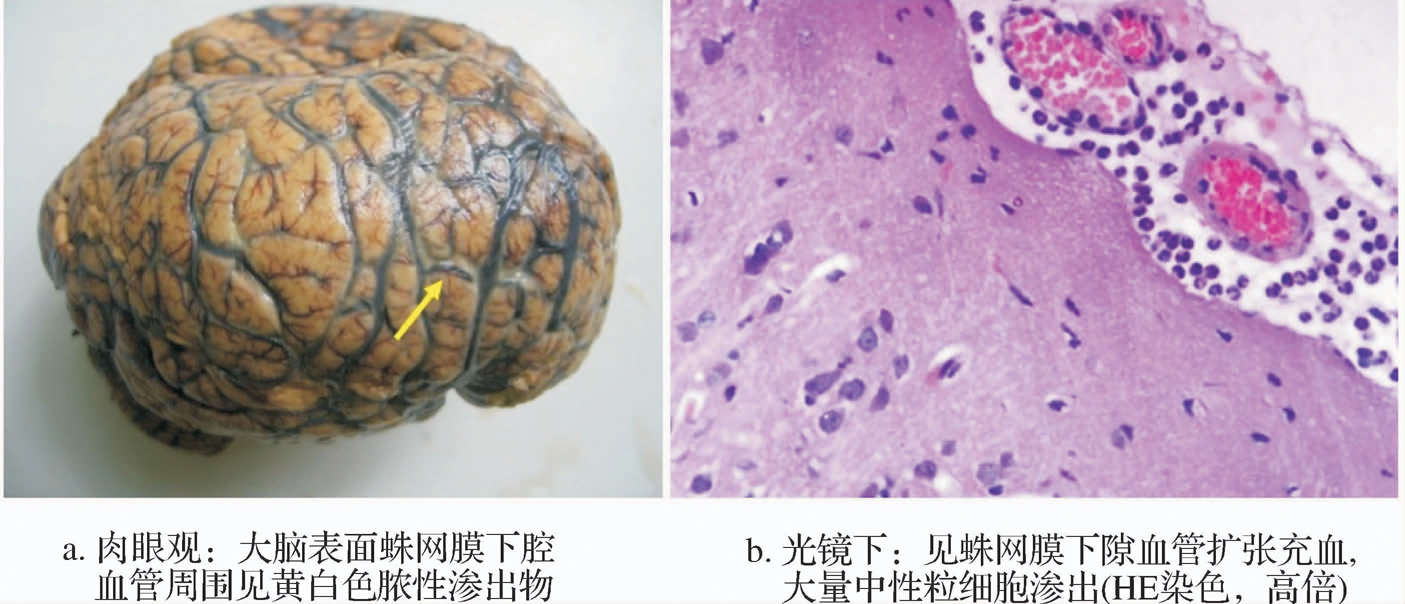
\includegraphics{./images/Image00217.jpg}
 \captionsetup{justification=centering}
 \caption{流行性脑脊髓膜炎}
 \label{fig13-1}
  \end{figure} 

\subsubsection{恢复期}

经治疗后体温逐渐降至正常,皮肤淤点、淤斑消失,溃疡结痂愈合;症状逐渐好转,神经系统检查恢复正常。一般1~3周内痊愈。

\subsection{临床病理联系}

上呼吸道感染期可有轻微发热,咽痛,鼻咽部黏膜充血和分泌物增多等症状。鼻咽拭子培养可分离出脑膜炎双球菌。败血症期因内毒素作用,患者常突发寒战、高热、头痛、呕吐,全身不适,表情呆滞或烦躁不安,白细胞增多等感染症状。

脑脊髓膜炎期常有下列神经系统的临床表现:

\subsubsection{脑膜刺激症状}

临床表现为颈项强直,屈髋伸膝征(Kernig征)阳性,严重病例出现角弓反张。由于炎症累及脊神经根周围的蛛网膜及软脑膜,使神经根肿胀并在通过椎间孔处受压,当颈部或背部肌肉运动时,牵引受压的神经根而产生疼痛,于是颈背部肌肉出现保护性痉挛,导致颈部强直,头略向后仰。婴幼儿因腰背部肌肉发生保护性痉挛,使脊柱向后弯曲,形成“角弓反张”体征。若腰骶节段脊神经后根受炎症波及而受压,在屈髋伸膝试验时,由于坐骨神经牵拉,使腰骶部神经后根受到刺激引起疼痛,而呈现Kernig征阳性。

\subsubsection{颅内压升高症状}

表现为剧烈头痛,喷射性呕吐,昏迷,惊厥,小儿前囟饱满等。这是由于脑膜血管扩张充血,脑脊液生成增多,蛛网膜下腔脓性渗出物堆积,同时蛛网膜颗粒因脓性渗出物阻塞,影响了脑脊液重吸收,引起颅内压增高。若伴有脑水肿则颅内压升高更显著。

\subsubsection{脑脊液改变}

脑脊液压力升高,呈不同程度混浊甚至为脓样。实验室检查:细胞数增多(含大量中性粒细胞),蛋白质含量增加,糖及氧化物减少;脑脊液培养或涂片均可发现脑膜炎双球菌。

\subsubsection{颅神经麻痹症状}

如耳聋、斜视、视力障碍、面瘫,这是由于颅底部脑膜的炎症累及始于该部的Ⅲ、Ⅳ、Ⅴ、Ⅵ、Ⅶ等颅神经所致。

\subsection{结局和并发症}

由于磺胺类药物和有效抗生素的广泛应用,大多数流脑患者急性期多能治愈,死亡率由过去的70%~90%下降到5%以下。少数可转变为慢性,还可造成以下后遗症:①脑积水,由于蛛网膜下腔渗出物机化,引起脑膜粘连,导致脑脊液循环障碍;②脑梗死,由于脑底部动脉炎,使其管腔堵塞,造成局部缺血。

少数病例(主要为小儿)起病急,病情重,死亡率高,称为暴发型脑膜炎。又分为以下3种。

\subsubsection{败血症型}

主要表现为败血症性休克,而脑膜的病变轻微。特点为起病急骤,突发高热,寒战,头痛,呕吐,严重者伴有严重的周围循环衰竭,血压下降,脉搏细弱,呼吸急促等症状。其发生机制主要是由于大量的内毒素释放入血,引起休克和弥散性血管内凝血,使病情进一步恶化。皮肤黏膜可出现广泛的淤点、淤斑,同时伴两侧肾上腺皮质大片出血,肾上腺皮质功能严重不足,称为华-佛综合征(Waterhouse-Friderichsen
syndrome)。

\subsubsection{脑水肿型}

除脑膜脑炎外,由于内毒素的作用,引起脑组织淤血,脑血管壁通透性增加,大量浆液渗出,导致严重脑水肿和颅内压增高,同时软脑膜下脑组织中有不同程度中性粒细胞浸润,甚至发生脑软化,严重颅内高压为本型特征。临床上突发高热,剧烈头痛,频繁呕吐,常有惊厥,甚至昏迷,严重者可形成脑疝,如颞叶沟回向小脑天幕裂孔嵌入形成海马沟回疝;小脑扁桃体向枕骨大孔嵌入形成枕骨大孔疝。

\subsubsection{混合型}

兼有上述两型的表现,是病情最重的一型,死亡率极高。

\section{流行性乙型脑炎}

\begin{framed}
{案例13-1}

{【病例摘要】}

患者,男,4岁,因发热、头痛、嗜睡3天,抽搐2次,于××年8月15日由外院转入院。患儿3天前开始出现发热、头痛,次日发热加重,体温达39.5℃,精神萎靡、嗜睡并发生抽搐(持续2~3分钟),立即送往当地医院,因有过轻微咳嗽,初步诊断为“上感、高热惊厥”,给予抗生素及对症治疗,今日患儿病情加重,再次发生抽搐(持续4~5分钟),急转我院。EP:体温40℃,神志尚清、精神萎靡,呈嗜睡状,呼之能醒,心肺(-),腹软,肝脾未扪及,四肢紧张。

{【问题】}

(1)该患儿最可能患了什么疾病?还应该做哪些检查?

(2)该患儿脑部可能有哪些病理变化?
\end{framed}

流行性乙型脑炎(epidemic encephalitis
B)是由乙型脑炎病毒引起的一种急性传染病,简称乙脑。病变主要在大脑,脊髓也可受累,病理特征是中枢神经系统的变质性炎症。本病起病急,病情重,死亡率高,临床上有高热、嗜睡、头痛、呕吐、抽搐、谵妄、昏迷等表现。儿童发病率高于成人,10岁以下的儿童占50%~70%,常在夏秋季流行。

\subsection{病因及发病机制}

乙型脑炎病毒是一种嗜神经性的RNA病毒。传染源为乙型脑炎病人及隐性感染者和受感染的家畜(猪、马、牛等)、家禽(鸡、鸭、鹅等)。蚊虫(包括库蚊、伊蚊和按蚊)是本病重要传播媒介,当带病毒的蚊虫叮人吸血时,病毒即随蚊虫的唾液侵入人体。乙型脑炎病毒进入人体后是否发病,不仅与病毒的毒力和数量有关,而且还取决于人体的免疫能力和血-脑屏障功能。免疫力强、血-脑屏障功能正常时,病毒虽进入人体血循环,但不能进入脑组织,故并不发病,仅表现为短暂的病毒血症,且最终被机体消灭,称为隐性感染。若感染仅限于轻度病毒血症而不发病,或很少发生中枢神经症状,则称为轻型。机体抵抗力低下,血-脑屏障功能不健全或发育不完善(多为10岁以下儿童),病毒则可通过血-脑屏障侵入中枢神经系统的神经细胞内进行繁殖。被感染的神经细胞表面有膜抗原存在,机体针对该抗原所产生的体液免疫和细胞免疫反应,引起神经细胞损害,是病变发生的主要病理基础。

\subsection{病理变化}

主要病变特点是脑脊髓实质的变性坏死。病变分布广泛,以大脑皮质、基底核、间脑、中脑最为严重,小脑、延脑及桥脑次之,脊髓(颈段)病变最轻。

\subsubsection{肉眼观}

软脑膜充血、水肿明显,脑回变宽,脑沟变浅。脑组织切面充血水肿,严重者可有点状出血及粟粒或针尖大小的灰白色半透明软化灶,呈散在分布或聚集成群。

\subsubsection{镜下观}

常见以下几种病变:

\paragraph{变质性病变}
为本病的特征性变化,病毒在神经细胞内生长、复制,破坏其结构和功能。轻者神经细胞肿胀,尼氏小体减少或消失,胞质内出现空泡,核偏位。重者神经细胞皱缩,胞质深染,核固缩、碎裂,甚至溶解消失。在变性坏死的神经细胞周围,常有增生的少突胶质细胞围绕,称神经细胞卫星现象(图\ref{fig13-2});若小胶质细胞侵入到坏死的神经细胞内,则称神经细胞被噬现象(图\ref{fig13-3})。小脑浦金野细胞的大量减少,也是本病突出表现。病变进一步发展,神经组织(神经细胞及神经胶质细胞等)灶性坏死后溶解液化,形成染色淡、疏松的圆形或椭圆形筛网状病灶,即软化灶形成(图\ref{fig13-4})。软化灶分布范围广泛,主要见于灰质或灰白质交界处。软化灶可被吸收或由增生的胶质细胞所取代,形成胶质瘢痕,或由增生的胶质细胞包绕,形成小囊肿。
\begin{figure}[!htbp]
	\centering
	\begin{minipage}[b]{0.45\textwidth}
		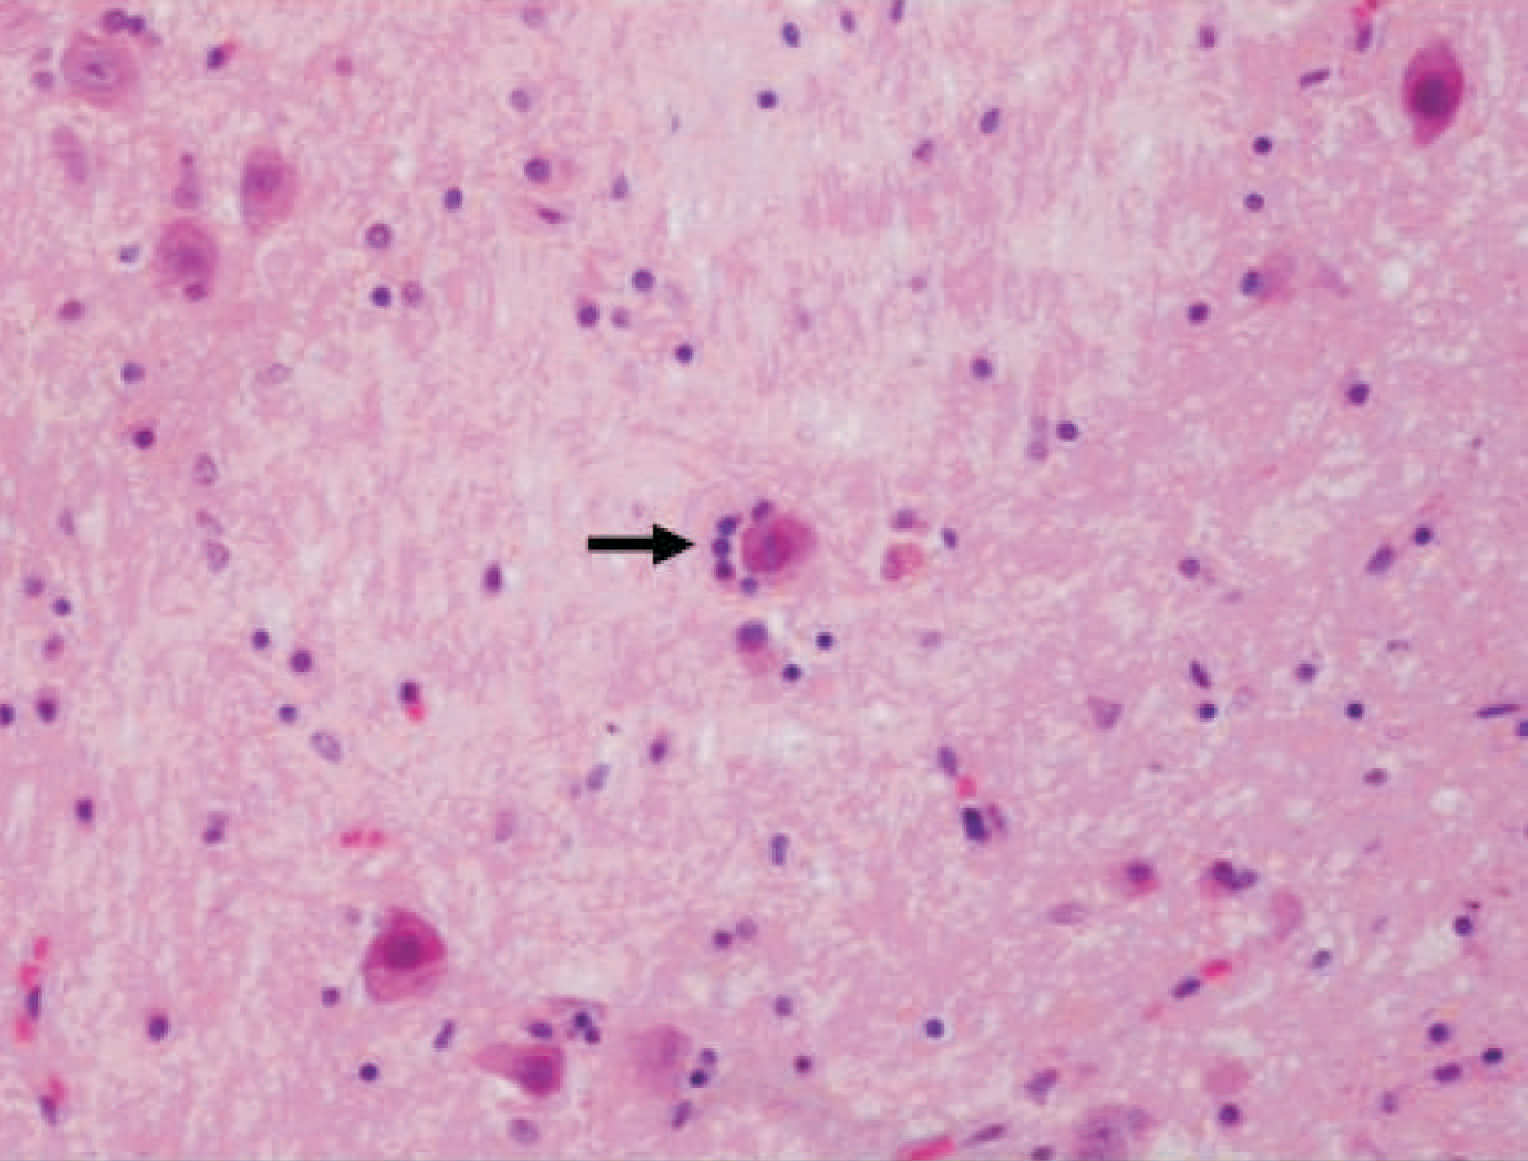
\includegraphics{./images/Image00218.jpg}
 \captionsetup{justification=centering}
 \caption{神经细胞卫星现象图(HE染色,中倍)}
 \label{fig13-2}
	\end{minipage}
	%	\end{figure} 
	%\FloatBarrier
	%\begin{figure}[!htbp]
	%    \centering
	\hspace{0.04\textwidth}%
	\begin{minipage}[b]{0.45\textwidth}
		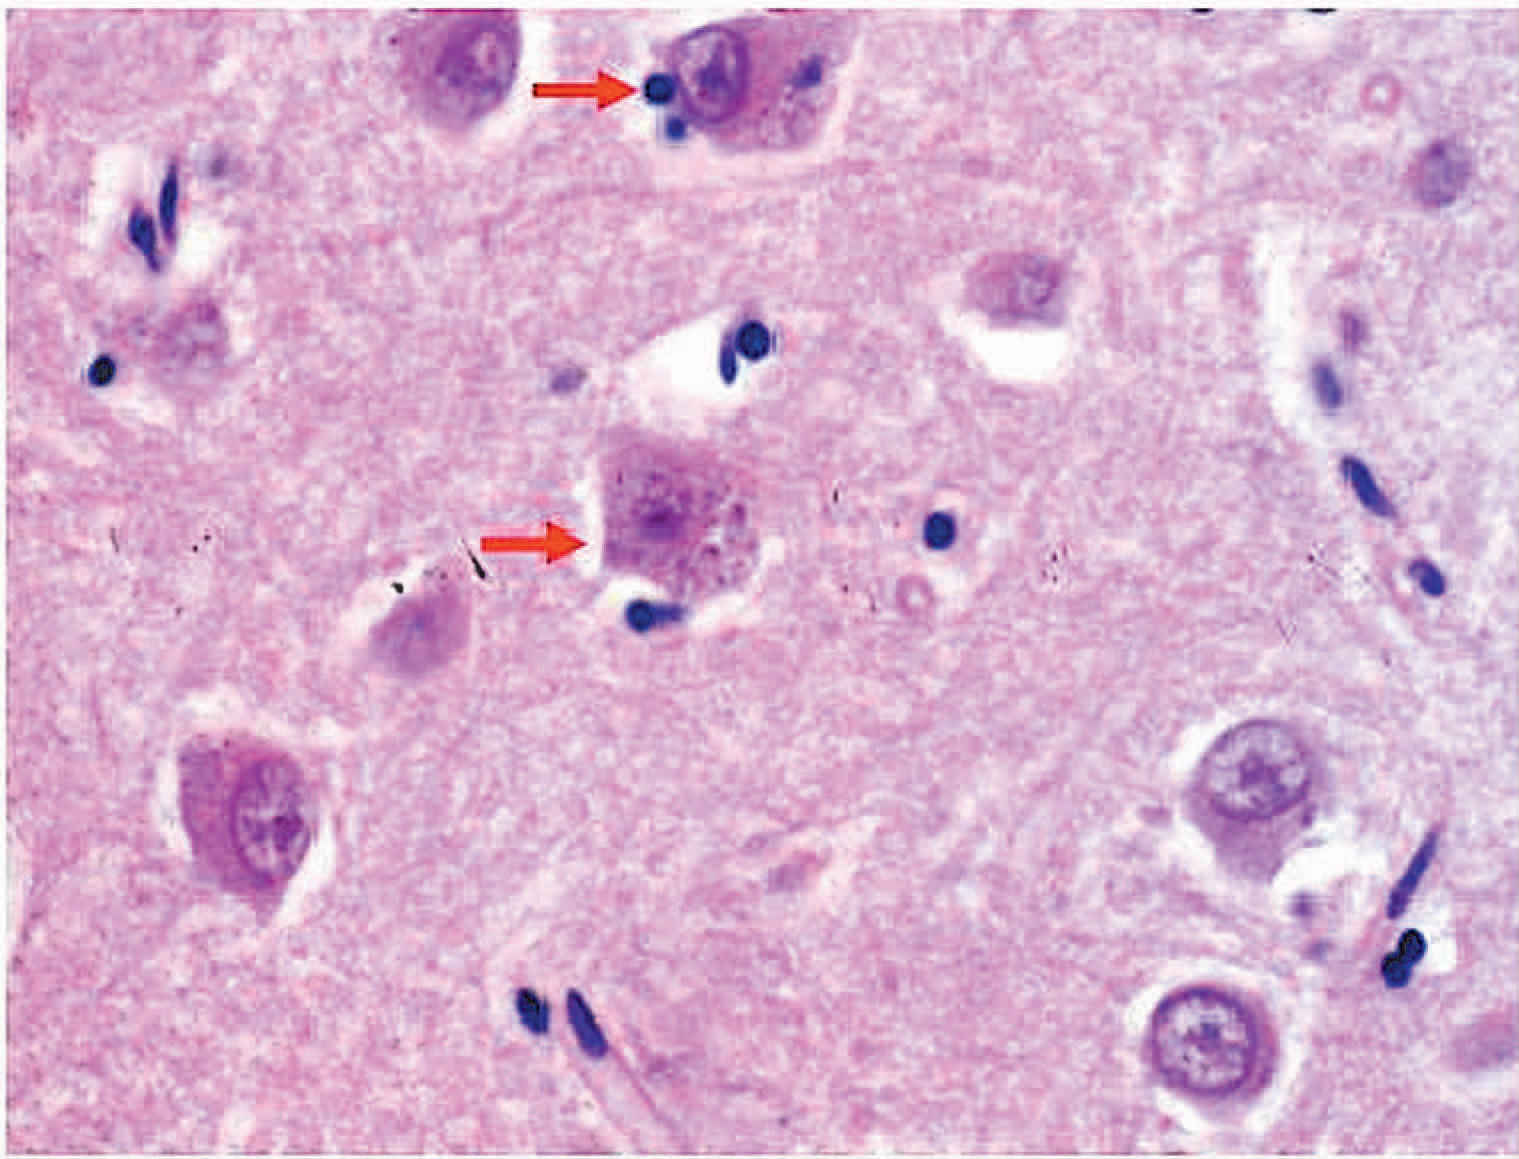
\includegraphics{./images/Image00219.jpg}
 \captionsetup{justification=centering}
 \caption{神经细胞被噬现象(HE染色,高倍)}
 \label{fig13-3}
    \end{minipage}
    \begin{minipage}[b]{0.45\textwidth}
		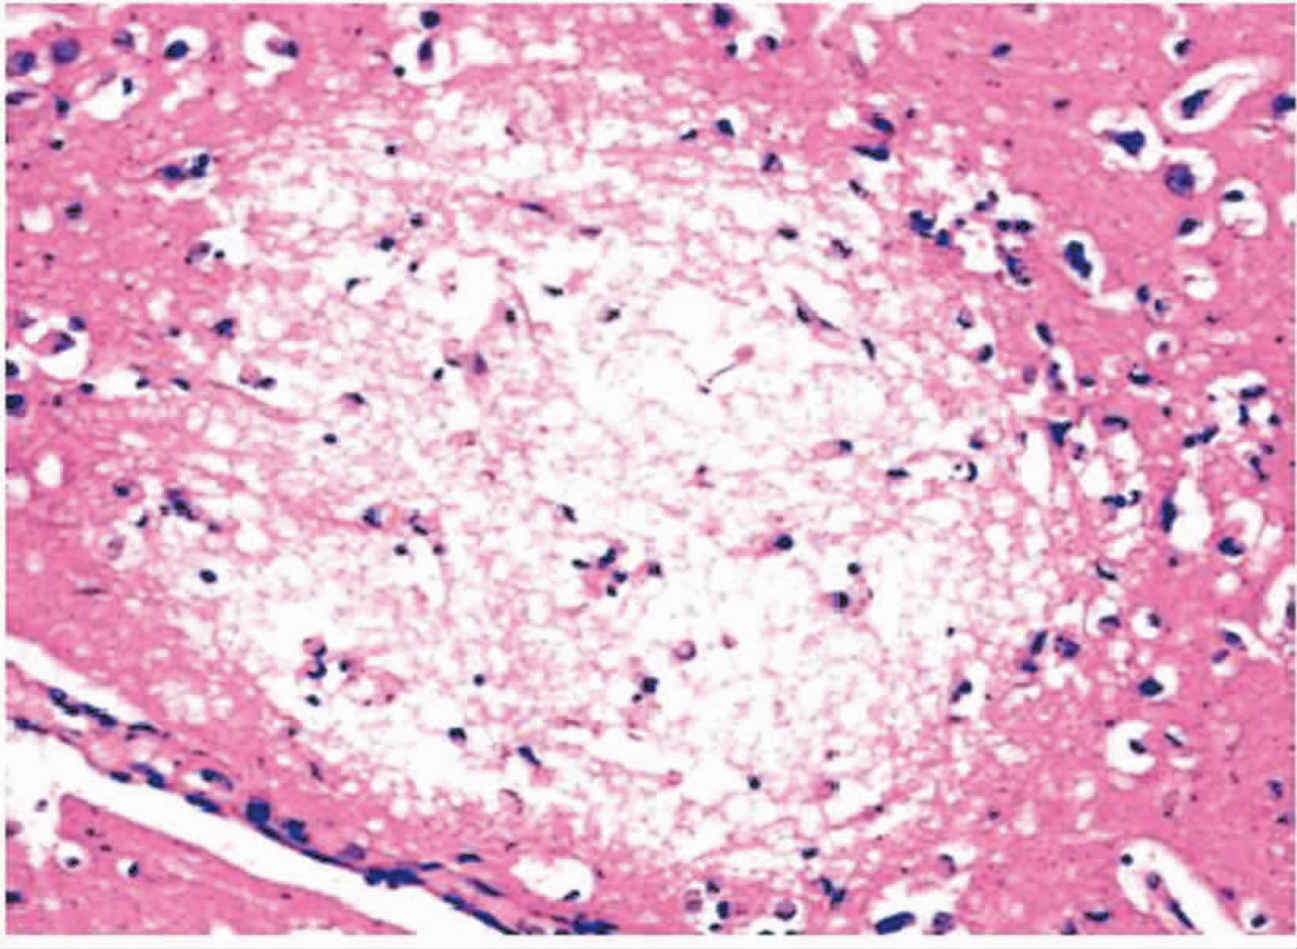
\includegraphics[height=.2\textheight]{./images/Image00220.jpg}
 \captionsetup{justification=centering}
 \caption{筛状软化灶图(HE染色,中倍)}
 \label{fig13-4}
	\end{minipage}
	%	\end{figure} 
	%\FloatBarrier
	%\begin{figure}[!htbp]
	%    \centering
	\hspace{0.04\textwidth}%
	\begin{minipage}[b]{0.45\textwidth}
		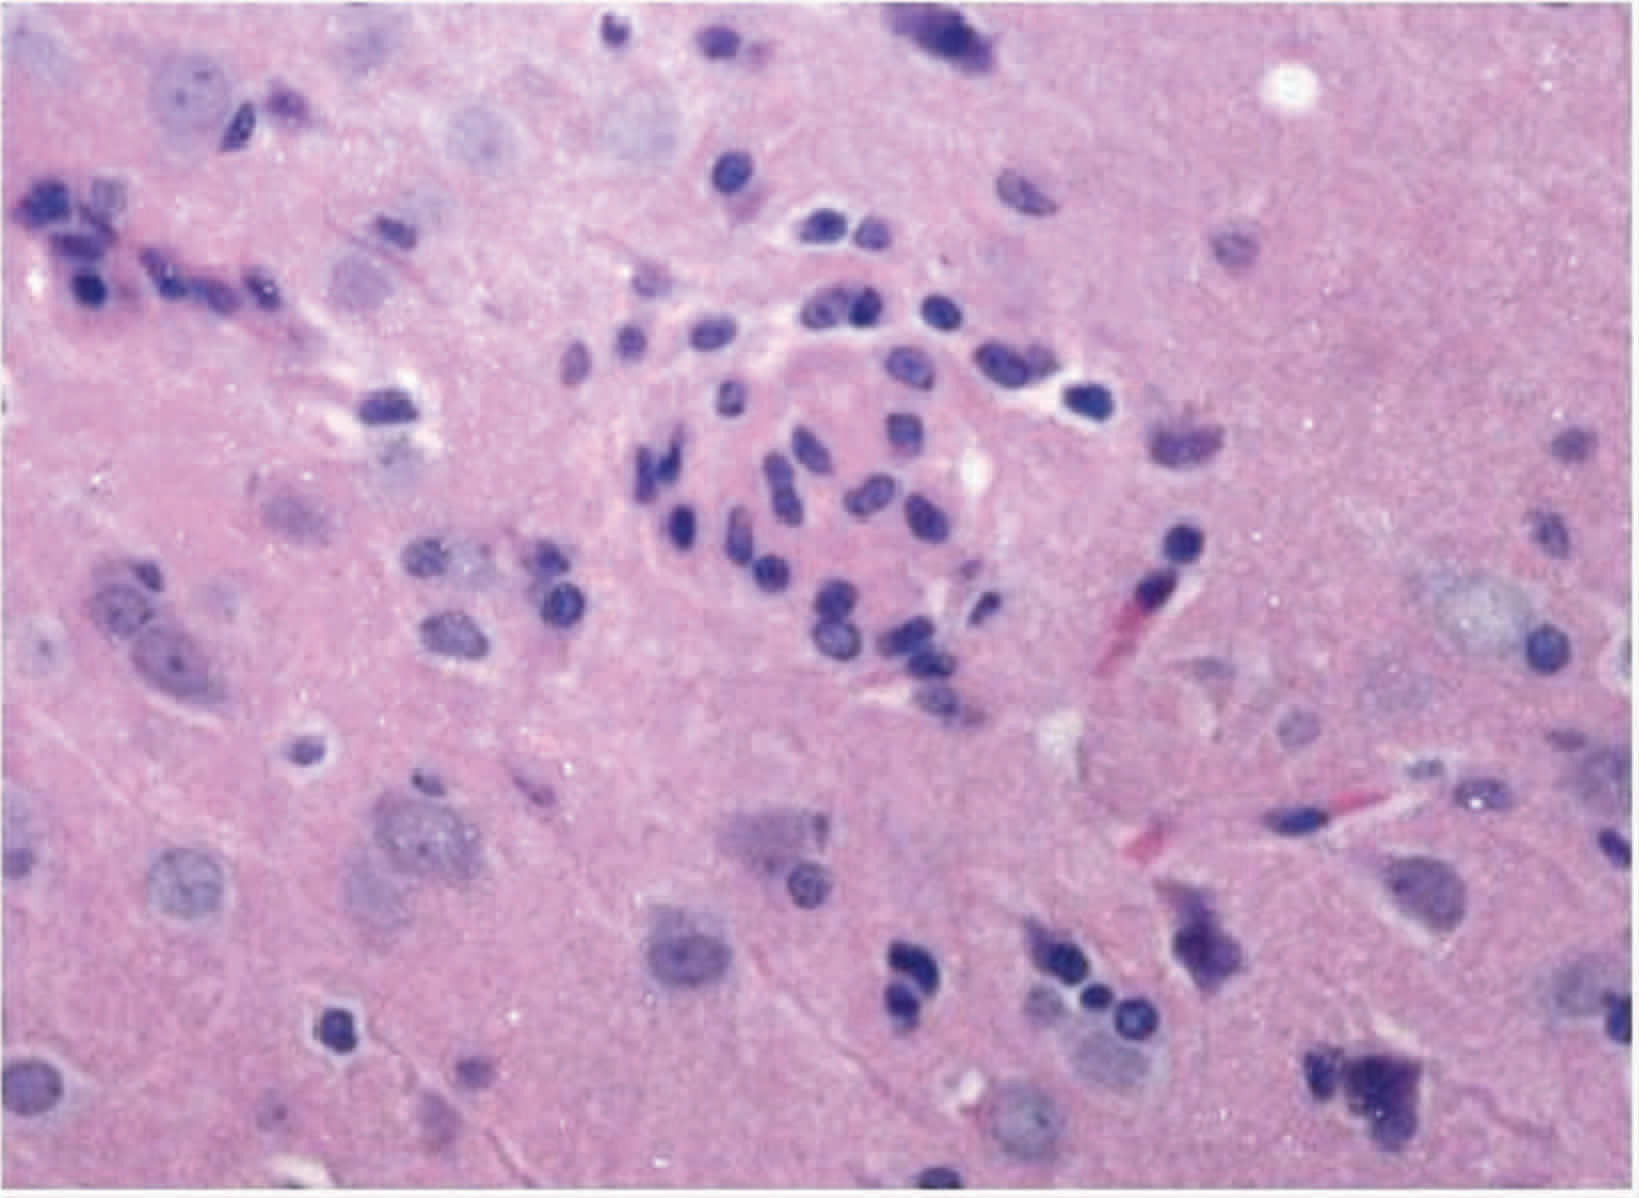
\includegraphics[height=.2\textheight]{./images/Image00221.jpg}
 \captionsetup{justification=centering}
 \caption{胶质细胞结节(HE染色,高倍)}
 \label{fig13-5}
	\end{minipage}
\end{figure}

\paragraph{渗出性病变}
脑实质血管高度扩张、充血,小静脉和毛细血管腔内可有透明血栓形成,有时可见小出血灶。血管周围间隙增宽,有浆液聚集,并有以淋巴细胞为主和少量单核细胞及浆细胞围绕在血管周围,形成袖套状浸润。

\paragraph{增生性病变}
主要为神经胶质细胞增生。小胶质细胞呈弥漫性增生或聚集成群,形成胶质细胞结节(图\ref{fig13-5}),常位于小血管旁或变性、坏死、崩解的神经细胞周围,最后形成胶质瘢痕,具有修复作用。

\subsection{临床病理联系}

早期可出现病毒血症症状,表现为高热、全身不适等。继而由于神经细胞广泛的变性坏死,出现嗜睡或昏迷。当脑内神经细胞受累严重时,可致上运动神经元损害,失去对下运动神经元的控制,引起肌张力亢进,发生临床上的抽搐痉挛,即所谓痉挛性麻痹。当脊髓前角运动神经元受损严重时,则出现肌张力降低,膝反射减弱或消失,重者可发生弛缓性麻痹。桥脑和延髓的运动神经元受损严重时,可出现延髓性麻痹,病人吞咽、说话困难,甚至发生呼吸困难、循环衰竭。由于脑血管扩张充血、血管内皮细胞受损,使血管壁通透性增高,可致脑组织水肿而引起颅内压增高,出现头痛,呕吐。严重脑水肿可形成脑疝,常见的有枕骨大孔疝和海马沟回疝。枕骨大孔疝时延脑呼吸中枢和血管运动中枢受挤压,可引起中枢性呼吸、循环衰竭,使患者死亡。由于脑膜可有轻度炎症反应,在临床上可出现轻度脑膜刺激症状。脑脊液检查:透明或稍混浊,细胞数增多(以淋巴细胞为主)。

\subsection{结局及并发症}

乙脑病人经中西医结合治疗,大多数病人可痊愈。少数病变严重的病例,康复时间较长,并可出现语言障碍、痴呆、肢体瘫痪等。如颅神经麻痹可发生吞咽困难、中枢性面瘫及眼球运动障碍等,这些情况在数月之后多能恢复正常;若病程超过6个月不能及时恢复则可留下后遗症。极少数严重病例,可因中枢性呼吸、循环衰竭或合并小叶性肺炎而死亡。

流行性脑脊髓膜炎与流行性乙型脑炎的鉴别见表\ref{tab13-1}。

\begin{table}[ht]
	\caption{流行性脑脊髓膜炎与流行性乙型脑炎的比较}
	\label{tab13-1}
	\centering
	\begin{tabular}{lp{5cm}p{5cm}}
	\toprule
	&流行性脑脊髓膜炎&流行性乙型脑炎\\
	\midrule
	病原体&脑膜炎双球菌&乙型脑炎病毒\\
	传染途径&呼吸道飞沫传染&以蚊虫为媒介经血传染\\
	流行季节&冬春季  &夏秋季\\
	病变特点&脑脊髓膜化脓性炎,脑脊髓膜高度充血,蛛网膜下隙充满大量脓性渗出物,脑实质病变不明显:&脑实质变质性炎.神经细胞变性坏死,软化灶形成,胶质细胞增生,脑血管扩张充血,形成淋巴细胞套 \\
	临床表现&脑膜刺激症状,颅内压升高症状,皮肤、黏膜出现淤斑、淤点&嗜睡、昏迷、抽搐等神经症状明显,可有颅内压增高,脑膜刺激不明显\\
	脑脊液检查&压力增高、浑浊,细胞数明显增多(主要为中性粒细胞),可找到细菌&透明或微混浊,细胞数轻度增加(多为淋巴细胞),细菌检查阴性\\
	结局&磺胺药及抗生素治疗预后好,暴发型脑膜炎死亡率高&少数较重病例常有后遗症\\
	\bottomrule
	\end{tabular}
\end{table}

\section{阿尔茨海默病}

阿尔茨海默病(Alzheimer
disease,AD)又称老年性痴呆,是一组原因不明的大脑原发性变性疾病,常发生于老年期或老年前期,多缓慢起病,病程呈进行性发展,临床上以进行性智能缺损为主要表现,包括记忆、智力、定向、判断、情感障碍等,导致行为失常,甚至发生意识模糊。随着人民生活水平的提高、人的寿命延长,老年人口的数量不断增加,此病的发病率日趋增高,已受到社会的关注。

\subsection{病因及发病机制}

本病的病因和发病机制目前尚不清楚。其发病的主要危险因素可能与高龄、家族遗传史、脑外伤、微量元素、慢性病毒感染等有关。目前研究认为本病发生的机制可能有:①淀粉样物质沉积:由于脑细胞代谢障碍,细胞膜表面一种具有受体样结构的跨膜蛋白异常降解,产生不能溶解的β淀粉样蛋白,该蛋白对脑细胞有毒性作用。②遗传因素:约有10%本病患者有遗传倾向,分子遗传学研究已发现了一些与本病有关的基因,如早老蛋白1、早老蛋白2、APP基因和载脂蛋白(APoE),分别定位于第14、1、21和19号染色体。③τ蛋白过度磷酸化:τ蛋白是神经细胞内的一种骨架蛋白,过度磷酸化可造成神经原纤维缠结,从而影响脑细胞的结构和功能。④受教育程度和经济水平:低教育和低收入者发病率较高,不断学习可降低本病的发病率。⑤继发性神经递质改变:主要是乙酰胆碱减少。

\subsection{病理变化}

\subsubsection{肉眼观}

脑明显萎缩,重量减轻,脑回变窄,脑沟增宽,尤以颞叶、顶叶及前额区的萎缩最明显。脑室扩大,脑脊液体积增加。

\subsubsection{镜下观}

脑实质普遍萎缩,脑细胞受损、丧失,神经元减少及轴索和突触异常。还可见以下几种改变。

\paragraph{老年斑}
脑实质内可见主要由淀粉样蛋白在细胞外沉积而成的老年斑,直径在20~150
μm,以海马回和额叶皮质多见,基底节、丘脑、小脑也有发现。HE染色呈嗜酸性;嗜银染色斑块中心为均一的嗜银团;免疫组化抗β淀粉样蛋白(A{4}
)抗体标记阳性;电镜证实是由多个异常扩张变性的轴突终末及淀粉样细丝构成。

\paragraph{神经原纤维缠结}
电镜下见神经原纤维增粗、扭曲,形成缠结,呈双股螺旋状缠绕的细丝,多见于额叶、颞叶皮质以及海马和杏仁核的锥体细胞。

\paragraph{颗粒空泡变性}
表现为神经细胞胞质出现成簇的空泡,内含嗜银颗粒,多见于海马的锥体细胞。

\paragraph{Hirano小体}
为神经细胞树突近端棒状嗜酸性包涵体,生化证实多为肌动蛋白,多见于海马的锥体细胞。

\subsection{临床病理联系和结局}

由于缓慢发生的脑容量下降,神经细胞代谢和神经递质改变等因素,导致病人出现记忆、认知和精神障碍,并可发生行为异常。记忆障碍常是本病的首发症状,初期以近事遗忘为主,其后则远事也遗忘。早期病人可出现主观任性、生活懒散、缺乏主动性、好猜疑,有时昼夜颠倒,注意力不集中;精神状态随病情发展而日益衰退,言语重复,动作幼稚,严重时外出后不认识家门,甚至连自己的名字也忘记;躯体方面,常出现偏瘫,癫痫发作,大小便失禁等;晚期可完全失去生活自理能力,失智并最终导致死亡。目前本病还无法治愈。

\begin{center}
    \textbf{知识链接}
\end{center}
\chapterabstract{现在认为β-淀粉样蛋白(Aβ)在大脑中过多积累是AD发病机制的核心。Aβ是一种可溶的、高度聚集的小分子多肽,分子量为4kDa,是淀粉样前体蛋白(APP)的水解产物。正常大脑含有极少量的Aβ,低浓度Aβ对未分化、不成熟的神经细胞有营养作用;而高浓度Aβ对已分化的、成熟的神经细胞则有毒性作用。在AD患者大脑内Aβ的产生和清除失衡,由于Aβ清除能力降低,大脑中Aβ浓度增高,并在细胞外沉积为老年斑,引起突触功能受损,最终导致神经细胞退行性变和痴呆。}

\section{帕金森病}
\begin{framed}
{案例13-2}

{【病例摘要】}

患者,男,72岁。因肢体震颤6年,伴行动迟缓3年,近来出现幻觉而前来就诊。既往史:高血压15年(治疗情况不详),无其他病史。体检:面具脸,行动迟缓,行走左侧不摆臂、拖步,颅神经未见异常,心、肺(-)。四肢静止性震颤4~6
Hz,左上肢最明显;四肢肌张力呈齿轮样增高:左上肢3级,左下肢2级,右上、下肢1级;四肢肌力Ⅴ级。腱反射正常,头颅MRI未见异常。

{【问题】}

(1)该患者中枢神经系统可能有哪些病理变化?

(2)试分析该患者临床表现发生的原因。
\end{framed}

帕金森病(Parkinson
disease,PD)又称原发性震颤麻痹,是一种常见于中老年的慢性神经系统变性疾病,病变以纹状体、黑质损害为主,多在50~80岁发病,起病缓慢,呈进行性加重。主要表现为动作缓慢,身体颤抖、四肢僵硬等。

\subsection{病因及发病机制}

本病的病因尚未明了。10%左右的病人有家族史;部分患者可因脑炎、脑动脉硬化、脑外伤、甲状旁腺功能减退等引起。此外,某些毒物(如一氧化碳、氰化物)、药物(如酚噻嗪类、抗忧郁剂)及微量元素(如锰、汞)也可引起类似的症状,称为帕金森综合征。其发病机制可能主要是由于多巴胺型神经元的变性,使多巴胺不足,而胆碱能神经相对亢进,引起神经功能紊乱。

\subsection{病理变化}

\subsubsection{肉眼观}

早期无明显变化,晚期可见中脑的黑质、桥脑的蓝斑和迷走神经运动核等处的神经色素脱失。

\subsubsection{镜下观}

黑质、纹状体神经黑色素细胞丧失,残留的神经细胞胞质中出现圆形、中心呈强折光、嗜酸性的Lewy小体。电镜证实该小体由中心致密、周围松散的细丝构成。

\subsection{临床病理联系和结局}

由于黑质神经细胞的脱失、变性,多巴胺合成减少,而乙酰胆碱相对较高,前者为抑制性神经递质,后者为兴奋性神经递质,两者平衡失调,从而引起相应临床表现。主要有:

\subsubsection{震颤}

多见于四肢和头部,以手部最明显,手指的颤抖呈“搓丸样”运动,每秒钟4~6次,开始为静止性震颤,晚期可呈持续性。

\subsubsection{肌肉僵硬}

这是因为伸肌、屈肌张力均增高,患者在松弛状态下被动运动时所遇阻力明显增大,有铅管样阻力感(铅管样强直),若同时伴有肢体颤抖可呈齿轮样感(齿轮样强直)。

\subsubsection{运动障碍}

由于肌肉僵硬,病人可以自我控制的随意运动减少,姿势步态不稳,起步止步艰难,发音困难,日常生活(如生活起居、洗漱、进食)不能自理。

其他还可有假面具样面容,易激动(偶有阵发性冲动行为),易出汗、多油脂,部分病人会出现顽固性便秘等与自主神经有关的症状。

某些晚期病人可出现痴呆症状。

PD本身虽然不是一种致命性疾病,但却可严重影响日常生活,甚至致残,给病人造成极大痛苦;晚期出现的并发症(包括肺炎、骨折、尿路感染等)则可成为导致死亡的直接原因。

PD与AD都是多发生于老年人的慢性疾病,病因和发病机制尚不明确,在病理变化和临床表现上区别还是明显的。AD与PD的鉴别见表\ref{tab13-2}。

\begin{table}[ht]
	\caption{阿尔茨海默病与帕金森病的比较}
	\label{tab13-2}
	\centering
	\begin{tabular}{lp{5cm}p{5cm}}
	\toprule
	&阿尔茨海默病&帕金森病\\
	\midrule
	病变部位&大脑皮质,以额叶、顶叶及颞叶最显著&中脑黑质、脑桥蓝斑、大脑基底核等\\
	肉眼观察&脑明显萎缩,脑回变窄,脑沟变深&黑质和蓝斑脱色素\\
	镜下改变&①老年斑;②神经原纤维缠结;③颗粒空泡变性;④ CHirano小体形成&a.黑色素细胞丧失;b.lewy小体形成\\
	临床表现&进行性痴呆,记忆、智力、定向、判断和情感障碍,行为失常甚至发生意识模糊&震颤、肌肉僵硬、运动障碍、姿势及歩态不稳、起步及止步困难、假面具样面容某些病人晚期可出现痴呆\\
	\bottomrule
	\end{tabular}
\end{table}

\section*{复习与思考}

{一、名词解释}

神经细胞卫星现象 神经细胞被噬现象 老年斑 lewy小体

{二、问答题}

1. 简述流行性脑脊髓膜炎的病理变化及临床病理联系。

2. 简述流行性乙型脑炎的病理变化及临床病理联系。

3. 列表比较流脑、乙脑的不同点。

4. 简述阿尔茨海默病的病变特点及临床病理联系。

5. 简述帕金森病的病变特点及病理与临床联系。

{三、临床病理分析}

刘某,男性,1.5岁。

主诉:发热、头痛2天,呕吐、抽搐、神志不清1天。

现病史:患儿2天前开始发热伴头痛、鼻塞,食欲不好,当地医院诊断为“感冒”,但治疗后未见好转。至昨日高热不退,频繁喷射状呕吐,反复发生惊厥,神志不清,今晨6:45入院。

体格检查:体温40.1℃,脉搏143次/分,血压76/48 mmHg(10.13/6.40
kPa),呼吸28次/分。急性病容,昏睡,唇、指端发绀,全身皮肤可见淤点、淤斑,局部呈片状,颈有抵抗;呼吸急促,心律齐,无杂音;全腹软,肝脾轻度肿大;Kernig征(+),Brudzinski征(+)。

实验室检查:血白细胞计数17$\times 10^9$ /L,中性粒细胞86%,脑脊液压力为294
mm\ce{H2O}(2.88 kPa),淡黄、混浊,细胞数1.4$\times 10^9$
/L,总蛋白1 960
mg/L,糖0.73 mmol/L,氯化物101
mmol/L,脑脊液沉淀和淤点采血涂片均查出革兰阴性双球菌。

治疗经过:入院后给予大量广谱抗生素及激素,纠正水、电解质紊乱及酸中毒治疗,但患儿血压时好时坏,进入昏迷状态,淤点、淤斑增多并融合,血压下降,于入院后47小时抢救无效死亡。

尸解摘要:呈轻度角弓反张状。大脑表面血管高度扩张、充血,蛛网膜下腔混浊不清,有较多灰白色脓性渗出物积聚;双肾上腺出血。两肺下叶散在灰白色病灶,镜下可见肺泡腔充满中性粒细胞,心肌横纹消失;肝细胞质内有的充满粉红色颗粒,有的出现脂肪空泡。

讨论题:

1. 根据以上资料应作何种诊断?为什么?

2. 试分析该患儿的死亡原因。

3. 本病例临床表现与病理变化之间有何联系?

4. 解释尸检所见的相关病理变化。